\chapter{数値実験}
\label{chap:experiment}

本章では,提案したアルゴリズムの有効性を検証するための実験を行う.
実験で比較するアルゴリズムは次の通り.
\begin{enumerate}
\item 再計算(Brandesのアルゴリズム)
  \par 辺が挿入または削除される度にBrandesのアルゴリズム(アルゴリズム\ref{algo:brandes})で媒介中心性を再計算する
\item 更新(提案手法)
  \par 辺が挿入された場合アルゴリズム\ref{algo:incremental-algorithm}で,削除された場合アルゴリズム\ref{algo:decremental-algorithm}で媒介中心性を更新する
\end{enumerate}

まず,人工ネットワークに対する実験を行う.ここでは,Brandesのアルゴリズムとの
比較や,更新したペア依存度の数と実行時間の関係,媒介中心性を更新した頂点数と
実際に媒介中心性が変化した頂点の関係を明らかにし,
\ref{subsect:computational-complexity-of-incremental-algorithm}と
\ref{subsect:computational-complexity-of-decremental-algorithm}で
行った理論的な解析結果との関連を示す.

次に,実ネットワークに対する実験を行う.ここでは,頑健な道路ネットワークの
構築と,媒介中心性のリアルタイム計算への応用を想定した実験を行う.

\section{人工ネットワークに対する実験}
\label{sect:exp-artificial}

本節では,以下の項目について実験を行い,その結果について考察する.
\begin{enumerate}
\item Brandesのアルゴリズムとの比較
\item ペア依存度を更新した頂点ペアの数と実行時間の関係
\item 媒介中心性が実際に変化した頂点の数と更新した頂点の数の関係
\end{enumerate}

この実験では,次の二種類の人工ネットワークを対象とする.
\begin{enumerate}
\item Erd\H{o}s--R\'{e}nyiモデル\cite{Erdos1959}
\item Barab\'{a}si--Albertモデル\cite{Barabasi1999}
\end{enumerate}

\subsection{Brandesのアルゴリズムとの比較}

図\ref{fig:exp-artificial-order}は各アルゴリズムの実行時間を比較したものである.
各ネットワークの平均次数はおよそ$4$である.それぞれの頂点数について,
100個のネットワークに対する実行時間の最大値および平均値を計算している.

\begin{figure}[tb]
  \centering
  \includegraphics{exp-artificial-order.pdf}
  \caption{頂点数に対する実行時間の比較}
  \label{fig:exp-artificial-order}
\end{figure}

図\ref{fig:exp-artificial-order}より,二種類のネットワーク全てに対して,
頂点数が増加するとともに更新の平均実行時間が再計算のものと比べて短くなっていることが分かる.
ペア依存度を再計算する必要がある頂点が頂点数の増加とともに比較的少なくなることが理由と考えられる.

\subsection{更新の量と実行時間の関係}

提案したアルゴリズムのようなオンラインアルゴリズムの性能を評価するためには,
アルゴリズムによって更新した要素の数を考慮する必要がある.
\cite{Ramalingam1996,Lee2012,Pontecorvi2014}
ここでは,ペア依存度を更新した頂点ペア数と実行時間の関係を実験によって
明らかにする.さらに,
\ref{subsect:computational-complexity-of-incremental-algorithm}と
\ref{subsect:computational-complexity-of-decremental-algorithm}で
行った理論的な解析結果と,実験データの挙動が一致するかを検証する.

図\ref{fig:exp-artificial-update}はペア依存度を更新した頂点ペア数と実行時間の関係を表す.
頂点数を$1000$,平均次数は$4$または$64$とし,$100$個のネットワークに対してそれぞれ$1$回の更新を行った.

\begin{figure}[tb]
  \centering
  \includegraphics{exp-artificial-update.pdf}
  \caption{更新した頂点ペアの数に対する実行時間}
  \label{fig:exp-artificial-update}
\end{figure}

図\ref{fig:exp-artificial-update}より,更新した頂点ペア数が少ないと,実行時間が短くなることが分かる.
さらに,次数が大きいと実行時間が長くなる.この性質は辺の数が増加すると実行時間も
増加することを示し,理論的な解析結果と一致する.

\subsection{媒介中心性を更新した頂点の数と変化した頂点の数の関係}

\ref{subsect:computational-complexity-of-incremental-algorithm}と
\ref{subsect:computational-complexity-of-decremental-algorithm}で
行った理論解析では,媒介中心性を更新した頂点の数と実際に媒介中心性が変化した頂点の数との
間の関係が不明なままであった.ここでは,その関係を実験的に明らかにする.

図\ref{fig:exp-artificial-phony}に,媒介中心性を更新した頂点の数と
実際に媒介中心性が変化した頂点の数の関係を示す.

\begin{figure}[tb]
  \centering
  \includegraphics{exp-artificial-phony.pdf}
  \caption{媒介中心性が変化した頂点数に対する,更新した頂点の数}
  \label{fig:exp-artificial-phony}
\end{figure}

実際に媒介中心性が変化した頂点の集合を$B_\delta$とする.
実験結果より,媒介中心性が変化した頂点数$\lvert B_\delta\rvert$と媒介中心性を
更新した頂点数$\lvert V_\delta\rvert$の間に,$c$を定数として
\[ \lvert V_\delta\rvert=c\lvert B_\delta\rvert \]
が成り立つと推測すると,
\ref{subsect:computational-complexity-of-incremental-algorithm}と
\ref{subsect:computational-complexity-of-decremental-algorithm}で
行った理論解析の結果は,それぞれ,
\begin{equation*}
  \begin{aligned}
    &\mathcal{O}(\lvert V_\delta\rvert\lvert E_\delta\rvert+\lvert V_\delta\rvert^2\log\lvert V_\delta\rvert) \\
    &\:=\mathcal{O}(\lvert B_\delta\rvert\sum_{v\in B_\delta}\lvert\mathcal{N}_G(v)\rvert+\lvert B_\delta\rvert^2\log\lvert B_\delta\rvert)
  \end{aligned}
\end{equation*}
となる.

\section{実ネットワークに対する実験}
\label{sect:exp-realnet}

本節では,実ネットワークに対する実験を行う.頑健な道路ネットワークの
構築と,媒介中心性のリアルタイム計算への応用を想定した実験を行う.

\subsection{頑健な道路ネットワークの構築}
\label{subsect:exp-road}

第\ref{chap:introduction}章でも述べたように,道路ネットワークの頑健性を
向上するには,道路の建設によって媒介中心性の最大値を最小化する必要がある.
そこで,この実験では,実際の道路ネットワークに辺を挿入することによって,
媒介中心性の最大値を最小化させる.

道路ネットワークはOpenStreetMap\cite{OpenStreetMap}を利用して独自に構築した.
実験で用いる道路ネットワークを図\ref{fig:road-okayama}に示す.
このネットワークは$12165$個の頂点と$14820$本の辺を有する.

\begin{figure}[tb]
  \centering
  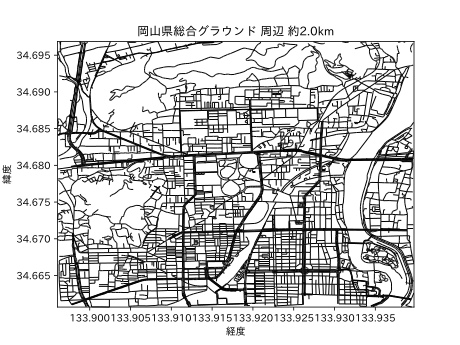
\includegraphics[width=.9\textwidth]{road-oka.pdf}
  \caption{実験で用いる道路ネットワーク}
  \label{fig:road-okayama}
\end{figure}

図\ref{fig:exp-road-oka-correlation}は,辺をひとつ追加したときの,
媒介中心性の最大値の分布である.
辺の追加によって,最大$0.1607$の正規化された媒介中心性を
$0.1379$まで減少させることに成功した.

また,辺追加によって媒介中心性の最大値が増加した例もある.
具体的に道路のどの部分に挿入すると媒介中心性が大きく減少,増加するかを
図\ref{fig:road-okayama-minmax}に示す.
図\ref{fig:exp-road-oka-correlation}と図\ref{fig:road-okayama-minmax}より,
媒介中心性が大きな頂点同士を結ぶと,媒介中心性の最大値が大きく変化することが分かる.

また,Brandesのアルゴリズムと提案手法それぞれの実行時間を比較した.
実行時間の累計を比較した図を図\ref{fig:exp-road-oka-time}に示す.
この実験において,提案手法はBrandesのアルゴリズムに比べおよそ$58$倍の性能をもつ.

\begin{figure}[tb]
  \centering
  \begin{minipage}{.45\textwidth}
    \includegraphics{exp-road-oka-correlation.pdf}
    \caption{辺挿入後の媒介中心性の最大値の分布}
    \label{fig:exp-road-oka-correlation}
  \end{minipage}\hfill
  \begin{minipage}{.45\textwidth}
    \includegraphics{exp-road-oka-time.pdf}
    \caption{実行時間の累計の比較}
    \label{fig:exp-road-oka-time}
  \end{minipage}
\end{figure}

\begin{figure}[tb]
  \centering
  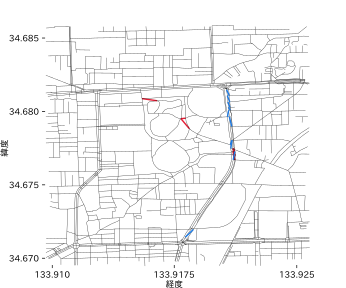
\includegraphics{road-oka-minmax.pdf}
  \caption{
    挿入すると媒介中心性の最大値を大きく変化させる辺 \\
    図\ref{fig:road-okayama}の拡大図である.
    青で示した辺は,挿入後の媒介中心性の最大値の減少量が大きい辺10本である.
    また,赤で示した辺は,挿入後の媒介中心性の最大値の増加量が大きい辺10本である.
  }
  \label{fig:road-okayama-minmax}
\end{figure}

\subsection{媒介中心性のリアルタイム計算}
\label{subsect:exp-sfhh}

第\ref{chap:introduction}章で説明したように,社会ネットワーク分析に
おいて,媒介中心性をはじめとした中心性に注目することは重要である.
しかし,現実の社会ネットワークでは,友人関係が時間とともに出現と消滅を繰り返している.
この実験では,友人関係の出現と消滅が頻繁に起こりうる状況で,
媒介中心性をリアルタイムで計算する用途への応用を想定する.

この実験では,SFHH\cite{Genois2018}というデータセットを用いた.
このデータセットは,ある会議の参加者に赤外線タグを持たせることによって,
参加者同士の交流の様子を記録したものである.

図\ref{fig:exp-sfhh}は,そのSFHHデータセットをもとに,辺の挿入と削除を
繰り返したときの,各手法の実行時間を表す.それとともに,20秒間の
うちに発生した,挿入と削除操作の内訳を示す.

\begin{figure}[tb]
  \centering
  \includegraphics{exp-sfhh.pdf}
  \caption{SFHHに対する実験結果}
  \label{fig:exp-sfhh}
\end{figure}

図より,小規模な場合ではあるが,媒介中心性をリアルタイムに計算できる.
しかし,更新の量が多い場合,Brandesのアルゴリズムの方が高速に計算していることが分かる.
今後は,多くの辺の操作に対応するアルゴリズムの開発が求められる.
